\documentclass[paper=a4,fontsize=11pt,twocolumn,pagesize,bibtotoc]{scrartcl}

\usepackage[utf8]{inputenc} 
\usepackage[T1]{fontenc}
\usepackage[english]{babel}

\usepackage[osf]{mathpazo} 
\usepackage{microtype}
\usepackage{tikz}
\usetikzlibrary{automata}
\usepackage{amsthm, amssymb, amsmath}
\usepackage{graphicx}
\usepackage{color}

\parindent0pt


\title{AppleMIDI}
\subtitle{Linux Kernel Driver Implementation}
\author{Felix Engelmann}

\begin{document}
	\maketitle
	
	As event based storage of music nearly disappeared completely from standard users, the 
	Musical Instrument Digital Interface
	is still the choice for digital instruments by professional musicians. The protocol is designed to transmit or store as many information as possible about the production of a tone. This normally includes the time at beginning of an event with the velocity of the beginning, which normally is related to the volume of the synthesized tone and a signal for the end, respectively the release of a key. Additionally to sound event transmission, there exists also a lot of control commands, e.g.: volume, balance, \dots
	Depending on the command, it is encoded by 2 to 4 bytes.
	
	By the original standard, the signals are transmitted via a special 5 pin cable. With the wide acceptance of USB an implementation of MIDI over USB arose quickly because it replaced the need for a dedicated port and enabled an convenient way to plug multiple devices to one computer through a hub. But then there are still restrictions of USB. A better and also established model for transmission is an IP based network which can be on top of any hardware layer.
	
	To accomplish that, a group at the University of Berkeley wrote an RFC for MIDI over RTP. Our Work was to enable this possibility in the linux kernel to interconnect linux computer with midi links.
	
	\section{Related Work}
	Along with the RFC 6295 there exists a small reference implementation by 
	J. Lazzaro, J. Wawrzynek
	with the core functionality, but they advise to not use it as a library. But it provides valuable insight for complex parts.
	
	To enable RTPMIDI on Windows,
	Tobias Erichsen
	provides a driver. As it is a commercial product, it os closed source and therefore not helpful in any way.
	
	With the wide distribution of tablets it got more and more common to replace expensive MIDI-pads with virtual ones or any other ideas of apps with which it is possible to create sounds and send them over the network to a synthesizer. On Android, the nmj is a closed source java library.
	
	The apple operating systems also include applemidi as part of the coreaudio framework.
	
	There are also two open source implementations. 
	Jascha Dachtera created an javascript version in nodejs. This has the advantage of high abstraction and provides a simple, easy to use interface. For building a bidirectional bridge, it is only required to implement receive hooks for each direction with one send cal to the other adapter.
	
	Im our test on the raspberry it served a good purpose as proof of concept to transfer midi over RTP. But due to the additional abstraction of the nodejs engine on the rather weak ARM, the processing time introduced a delay of about 6\,ms. This is too long for live performances.
	
	To get rid of the abstraction induced delay, 
	 Jonas Pommerening 
	implemented a universal adapter or alsa and RTP Midi directly in C. It is designed to be used in user-space applications with a run-loop to provide connectivity in non-blocking way. This is the code base of our driver, as all the management and book-keeping functions can be used as-is in the kernel.
	
	\section{RTPMIDI}
	The original (RFC 4695) as well as the updated RFC 6295
	%TODO: cite
	are only specifying the transmission of MIDI commands as payload of a Real Time Protocol packet. this is transmitted within a UDP datagram. But it does not include a specification for the session management. It only refers to using some sort of session description protocol
	(RFC 4566), e.g. SIP, which is also used to initiate phone and video calls over RTP.
	
	
	To minimize the divergence of combinations ant the resulting incompatibilities, Apple decided to use a standardized session session protocol. This is closely coupled to the RTPMidi transmission. Unfortunately the author decided to not publish the specification, however it found a broad acceptance. Because it is very simple, it was reverse engineered and there even exists a wireshark dissector to monitor the packets and their content.
	
	The state-machine of the session management is depicted in figure \ref{fig:state}.
	
	\begin{figure}
		\centering
		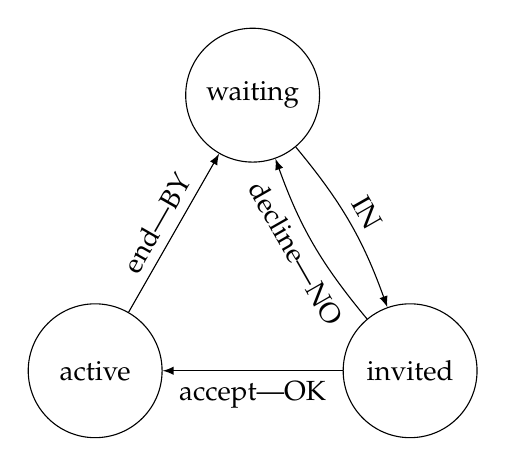
\begin{tikzpicture}[node distance=3cm,bend angle=10]
	        \node[state,minimum size=1.7cm] at (0,0)   (wait) {waiting};
	        \node[state,minimum size=1.7cm] at (2,-3.5)  (in) {invited};
	        \node[state,minimum size=1.7cm] at (-2,-3.5)  (act) {active};
		
			\path[-latex] (wait) edge[bend left] node[sloped,above] {IN} (in)
							(in) edge node[sloped,below] {accept|OK} (act)
								edge [bend left] node[sloped,below] {decline|NO} (wait)
							(act) edge node[sloped,above] {end|BY} (wait);
			%\path[-latex] (press) edge [loop below] node {$b_2|$on\&off} ();
			%\path[-latex] (act) edge [loop left] node {$\neg b_1|$off} ();
		\end{tikzpicture}
		\caption{state-machine of applemidi}
		\label{fig:state}
	\end{figure}
	
	The Applemidi communicates over two consecutive ports where an invitation and termination is required for both. The lower, normally even, default 5004, port is used for control commands. These include feedback, which provides the functionality of acknowledging received commands by the sequence number. The upper port is used for synchronization and the RTP connection.
	
	Parameters as the time-divisor
	which are otherwise exchanged at session invitation are kept fix at predefined values.
	
	\section{Global Structure}
	
	As most of the code-base was ported from the midikit project, it dictated the global structure of the driver. As it should act like a bridge, it is connected to the sequencer core for receiving midi commands and provides a listening network socket, where peers can subscribe and receive data. There is a handler for each interface to accept and forward or process the received events.
	
	During initialization of the module, the sockets are set up and the connection as a virtual midi output device is created. In addition, internal data structures are allocated to store information about the driver itself, as well as a list of connected peers. All these structures are freed on removal. This includes the proper disconnection of all active peers.
	
	\subsection{Networking}
	
	Networking in the kernel can be done for multiple purposes. For our use-case it is only necessary to get a very height level access to the networking stack. 
	
	Handling with network clients normally does not require to be in kernel-space. Even further, running complex sever functionality in the kernel can introduce severe security issues. If there is a remote exploit for this module, there are no right barriers ant the attacker has immediately full access to the whole system. The wise spread apache server even forks a complete new process with its own address space to separate each request. With this, a compromised request can not influence or damage the complete system easily.
	This encapsulation is not possible in the kernel, as all modules run in the same memory space without any shielding. Nevertheless it is possible to create a server as a module.
	
	For a convenient way to interoperate with the networking stack, the netpoll api offers all necessary functionality. An other way to create a socket is by using the system calls which are also used from user-space. Concerning performance, all three options are orders of magnitude faster than the delay of the actual ethernet transmission over the link. But there exists cases, for example it there is no user-space management on very small embedded devices, where it is necessary to use the kernel version.
	
	\subsubsection{Sockets}
	
	Within the kernel the opened sockets are not handles by file descriptors, but directly by a pointer to the \texttt{struct socket}. Instead of calling select from user-space to be notified when data is ready to read, a callback function can be set directly as a struct member. It is called in an asynchronous context whenever a packet with the specifies properties is received. In our case this means, that we only want Datagram, IPv4 packets. Because the socket is bound to a specific port, only packets arriving there are reported.
	
	For the control and the data socket, the same callback function is used, because the processing does not differ very much and differences can be caught, because the receiving socket is passed as an argument.
	
	A problem of the callback function is, that it only has the number of received bytes and a socket as parameters. There is so far no known method to pass a custom pointer to the callback function. Meanwhile the global variable, which is created at initialization and freed on exit, is accessed. Within this scenario, this imposes no problems to any functionality but is against the desired encapsulation of information.
	
	\subsubsection{Packet Processing}
	
	Up on arrival of a network packet, the first step is to get the according \texttt{struct sk\_buff} and test, if it is a valid packet. As the skb contains references for all fields of the packet, the source IP and port can be determined. This is needed to eventually add it as a peer. To distinguish AppleMIDI messages from others, the characteristic first 16 bits must be set to one and then be followed by one of the valid command types in two character ascii. To avoid malicious reads in memory, the length, encoded in the UDP header, is checked to fit the command length.
	
	The different commands are then further analyzed and processed. Invitations are always accepted and session terminations lead to removal of the peer. In a more advanced implementation, one could imagine , that if no alsa producer is connected, AppleMIDI invitations are rejected. All reactions that need to respond with a packet fill a \texttt{struct command}, which serves as the local representation of any AppleMIDI command.
	
	\subsubsection{Transmission} 
	
	After filling the command accordingly, it is assembled into the binary format. This is embedded in a UDP frame and IP packet with the destination of the peer. To enqueue the complete packet for transmission, \texttt{sock\_sendmsg} is called. As the data resides in the kernel space and system-calls check, that their data comes from user space, this has to be adjusted with \texttt{get\_fs} and \texttt{set\_fs}. 
	
	With this functionality of the driver, peers are able to connect and disconnect and a list of active peers is managed.
	
	To add the possibility to detect ungraceful disconnects, a sort of keep-alive ping is needed. This can be combined with the need to synchronize transmitter and receiver. In intervals of several seconds each side initiates a timing handshake. As every network time protocol, it is used to determine the clock of a remote machine over a network with latency. With a three-way handshake, the latency and the remote clock can be determined and sustained with high enough accuracy.
	The logic behind the synchronization is to exchange timestamps and delta differences to estimations of the remote clock. It was ported as-is from the midikit implementation.
	
	When run in a runloop, these synchronization tasks could be done in idle circles of the application. In the kernel, periodic tasks are managed with timers. As a resolution of seconds is enough, a standard timer based on jiffies was used.
	
	\subsection{Locks}
	
	As there exists already two callback functions which access the same structures, race conditions can occur and have to be mitigated. Considering the low probabilities of simultaneous timer and network events, this can be caught by a spinlock, which is part of the global management structure. Instead of spinning at a reception of a packet or a timeout, it only tests and skips it the lock is hold. This can be done safely, because packets can be lost in the network, which has the same effect as dropping them at the receiver. No realtime critical packets are received but only transmitted. Missed synchronizations will be retried at the next timeout.  
	
	\section{alsa}
	
	To be able to receive MIDI events, it is necessary to register the module at the sequencer core of the alsa framework. This is done in two steps. First a new virtual sound card must be allocated, which then can host a client. The client can be configured with multiple flags. As our driver should only receive commands, only the input flags are set.
	
	On arrival of data, the driver is notified by a callback function. There is a custom argument, so the driver management object hast not to be accessed from a global variable.
	
	In the current development status, every event is converted into an internal storage format of MIDI events and handed over to the transmission chain. In a subsequent version, this might be improved. An RTPMIDI packet can transport multiple commands with individual time offsets. This can be utilized by queueing events for a short time and then send multiple at once. The tradeoff between delay and throughput has to be chosen wisely. A common user case is playing an accord which should not result in many small packets but one big.
	
	The queue of commands is then first encoded as binary format. There, an other technique, known as running status, is used to increase throughput. If multiple consecutive commands are of the same type, the type is only needed for the first one and can be omitted for the rest. For example would multiple note-ons result in one complete command the the following containing only note and velocity.
	
	The RTPMIDI is then embedded into a RTP packet and finally sent in a UDP datagram to all peers.
	
	
	\section{Conclusion}
	
	The AppleMIDI driver is the choice for building digital music instruments with low power devices. It provides connection to a wide range of applications on all common operating systems.
	
	The use of a kernel module instead of a well separated user space program is only justified if there is not enough computation power. An example setup might be on a raspberry pi with the cmidid module for keys attached to gpio.
	
	Over all, it demonstrates the possibility and straightforwardness of porting a complex user space program to the kernel without libc including networking and sound connections.
	 
	
	
	
\end{document}